\documentclass[11pt, a4paper]{article}
\usepackage[utf8]{inputenc}
\usepackage[T1]{fontenc}
\usepackage{framed}
\usepackage[french]{babel}
\usepackage{tabularx}
\usepackage[T1]{fontenc}
\usepackage{lmodern}
\usepackage{graphicx}
\usepackage{fancyhdr}
\usepackage{amsfonts}
\usepackage{verbatim}
\usepackage{listings}
\usepackage{float}

\newcommand\defeq{\mathrel{\stackrel{\makebox[0pt]{\mbox{\normalfont\tiny def}}}{=}}}

\pagestyle{fancy}
\renewcommand\headrulewidth{0pt}
\fancyhead[L]{\emph{Groupe Amuat - Maalel - Poleya}}
\fancyhead[R]{Projet Logiciel Transversal}
\fancyfoot[L]{\emph{Rapport de Jalon 1}}
\fancyfoot[R]{\today}
\begin{document}

\title{Rapport de jalon de Projet Logiciel Transversal}

\maketitle

\tableofcontents
\newpage
 
\section{Objectif}

\subsection{Présentation générale}

L’objectif de ce projet est la réalisation d’un jeu de plateforme inspiré de “Dofus”, avec des règles et des designs simplifiés

\subsection{À propos du jeu}

\subsubsection{Règles du jeu}

Ce jeu possède deux modes: un mode exploration et un mode combat. Le joueur se déplace librement sur la carte en mode exploration et peut passer un mode combat en décidant d’affronter un ennemi présent sur cette même carte en cliquant dessus. La finalité de ce jeu d’aventure est de combattre des ennemis afin de gagner en expérience et de là augmenter de niveau.

\subsubsection{Description générale}

Voici la description générale du jeu à réaliser :

\begin{enumerate}
\item Deux modes : 
	\begin{enumerate}
		\item Mode exploration
		\item Mode combat
	\end{enumerate}
\item Des acteurs jouables et non jouables
	\begin{enumerate}
		\item Deux personnages (féminin, masculin)
		\item Cinq créatures (ennemis)
	\end{enumerate}
\item Six plateformes
	\begin{enumerate}
		\item Trois cartes pour le mode exploration
		\item Trois cartes pour le mode combat (générées à partir des cartes d'exploration)
	\end{enumerate}
\item Trois menus
	\begin{enumerate}
		\item Démarrer (Nouvelle partie, création de Personnage ...)
		\item Pause (Quitter, sauvegarder ...)
		\item Infos Personnage
	\end{enumerate}
\end{enumerate}

\subsubsection{Description détaillée}
Modes : 
\begin{itemize}
\item Exploration: Dans ce mode le joueur peut se déplacer librement sur la carte en cliquant sur une case, lancer un combat en se dirigeant vers une créature présente sur la carte.
\item Combat: Dans ce mode il s’agit d’un duel entre le joueur et une adversaire (créature/monstre). Ce mode prend fin lorsqu’un des acteurs  meurt.\\*
\end{itemize}


Voici la description détaillée du jeu à réaliser :

\begin{figure}[h]
  \centering
  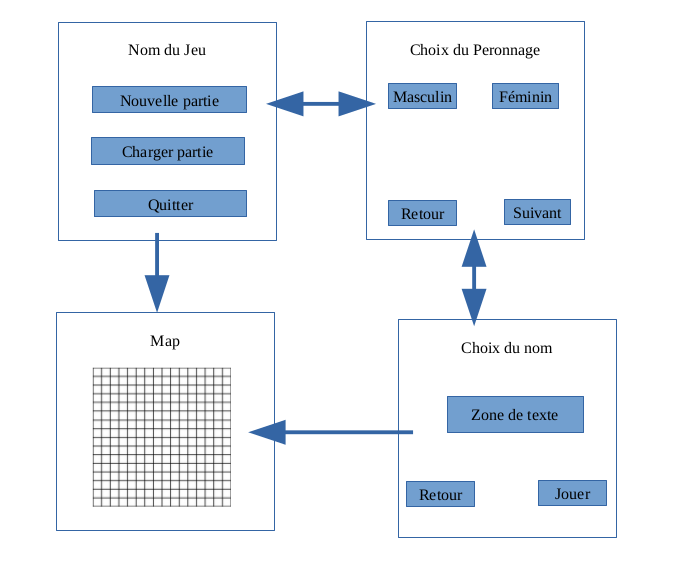
\includegraphics[scale=0.5]{img/MenuDemarrer.png}
  \caption{\emph{Organisation et maquettes des menus}}
\end{figure}

Au lancement du jeu, le menu démarrer s’affiche et trois options sont disponibles. Le bouton “Nouvelle partie” permet de lancer une nouvelle partie et redirige l’utilisateur vers un menu nommé “Choix du personnage. Le bouton “Charger partie” permet de lancer une partie enregistrée auparavant et redirige l’utilisateur vers la carte du jeu. Le bouton “Quitter” permet de mettre fin à l’exécution du jeu.
Dans le menu “Choix du personnage”, deux choix s’offrent à l’utilisateur soit un personnage masculin ou soit un personnage féminin. Une fois cette sélection effectuée l’utilisateur est dirigé vers un menu nommé “Choix du nom” permettant d’attribuer un pseudo au personnage retenu. Enfin, le bouton “Jouer” présent dans ce menu permet d’accéder à la plate-forme de jeu.

Menu Pause : 

\begin{figure}[h]
  \centering
  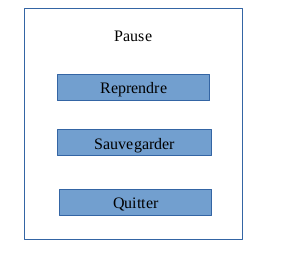
\includegraphics[scale=1]{img/MenuPause.png}
  \caption{\emph{Menu de pause}}
\end{figure}

Au cours du jeu (hormis en mode de combat) via le bouton ‘échap’ du clavier, l’utilisateur peut accéder au menu “Pause” qui propose à ce dernier trois options: reprendre la partie du jeu en cours, sauvegarder la partie de jeu en cours et quitter le jeu en cours. \\*

Menu Infos personnage : 

\begin{figure}[H]
  \centering
  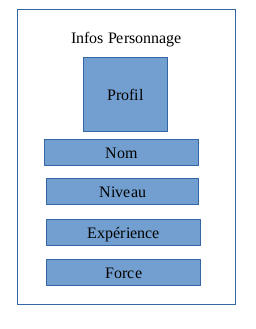
\includegraphics[scale=1]{img/MenuInfosPerso.png}
  \caption{\emph{Menu Infos}}
\end{figure}

Au cours du jeu (hormis en mode de combat) via le bouton ‘tab’ du clavier, l’utilisateur peut accéder au menu “Infos Personnage” qui contient tous les informations (nom, niveau, expérience, force, profil) sur le personnage du joueur.\\*

Cartes :

Deux types de cartes sont présents dans ce jeu : trois cartes dédiées au mode exploration et trois cartes dédiées au mode combat.

\begin{figure}[H]
  \centering
  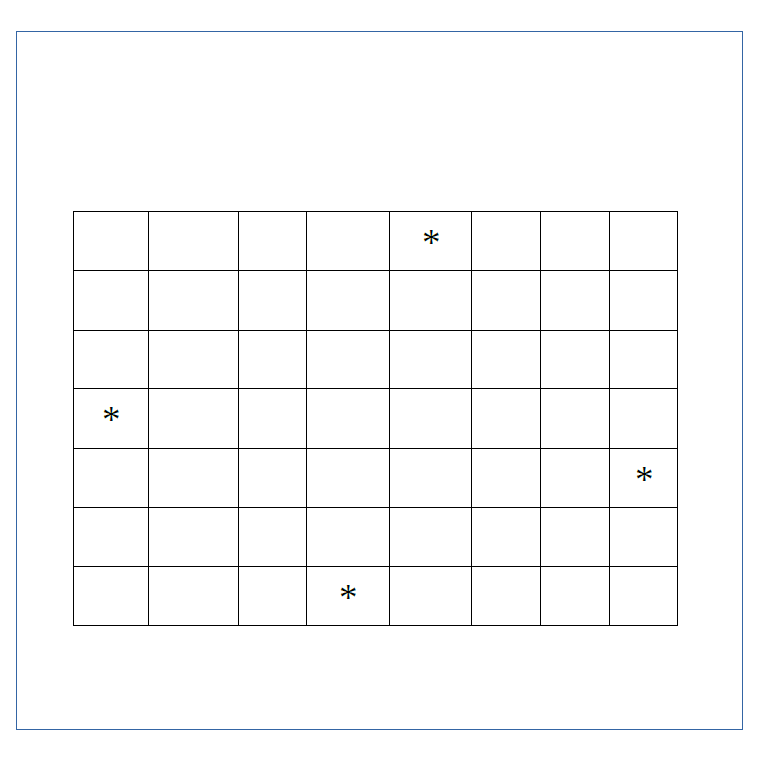
\includegraphics[scale=0.7]{img/CarteExplo.png}
  \caption{\emph{Modèle de carte en navigation}}
\end{figure}

\begin{itemize}
\item Le changement de carte s’effectue via les points d’accès (*)
\item Sur la carte exploration, il y a présence du personnage (joueur) et des ennemis (créatures)\\
\end{itemize}

Carte de combat :

\begin{figure}[H]
  \centering
  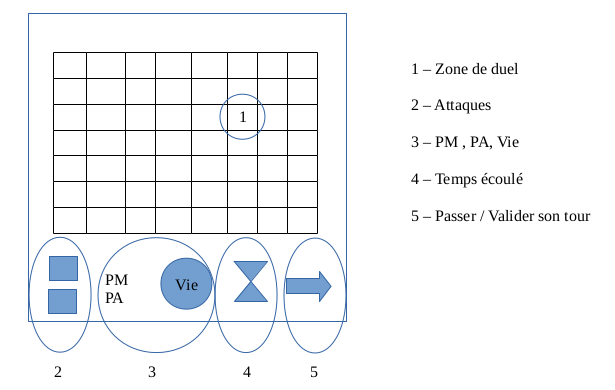
\includegraphics[scale=0.5]{img/CarteCombat.png}
  \caption{\emph{Modèle de carte en combat}}
\end{figure}

Sur la carte combat, il y a deux principales zones :

\begin{itemize}
\item Une zone de combat : 
	\begin{itemize}
	\item Dimension de la zone de duel : 12 carreaux * 10 carreaux
	\item Effets visuels: Assombrissement du fond et zoom sur la zone de combat
	\item Effets sonores: changement de musique
	\end{itemize}
\item une zone commandes/actions :
	\begin{itemize}
	\item une attaque corps à corps
	\item une attaque à distance
	\item Points de Mouvement (nombre de cases pouvant être parcourues par tour), Points d’Action (nombre d’attaques pouvant être lancées par tour) et Points de Vie dépendent du niveau du joueur
	\item Temps de jeu par tour de 60 secondes
	\item Touche “Passer/Valider” permet de mettre fin à son tour
	\end{itemize}
\end{itemize}

Les différents acteurs présents dans ce jeu sont :
	
\begin{itemize}
\item Deux personnages: un masculin et un féminin
\item Cinq créatures (I.A)
\end{itemize}

Le joueur augmente de niveau en faisant des duels et en gagnant de l’expérience et les créatures ont des niveaux différents allant de 1 à 10.\\*

Evolution du personnage :\\*

\begin{tabular}{|c|c|c|c|c|c|}
\hline
	Niveau & Vie & PM & PA & Exp \\
\hline
   1 & 100 & 3 & 6 & 100 \\
\hline
   2 & 150 & 4 & 7 & 200 \\
\hline
   3 & 200 & 5 & 8 & 300 \\
\hline
   4 & 250 & 6 & 9 & 400 \\
\hline
   5 & 300 & 7 & 10 & 500 \\
\hline
   6 & 350 & 8 & 11 & 600 \\
\hline
   7 & 400 & 9 & 12 & 700 \\
\hline
   8 & 450 & 10 & 13 & 800 \\
\hline
   9 & 500 & 11 & 14 & 900 \\
\hline
   10 & 550 & 12 & 15 & 1000 \\
 \hline 
\end{tabular}\\ \\*

Ce tableau résume l’évolution des paramètres Vie, PM, PA et Exp en fonction du niveau du personnage.\\*

\section{Description et conception des états}

\subsection{Description des états}

Notre jeu consiste principalement au déplacement d’un personnage sur une carte et à l’affrontement de monstres sur cette même carte. Le jeu évolue d’un état à un autre et cela de manière continue en fonction des actions du joueur. Ces différents états sont décrits de manière globale dans les paragraphes suivants.

\subsubsection{Etat Général}

Un état de jeu est formée par un ensemble d’éléments mobiles (heros, monstres) et d’un ensemble d’éléments fixes (cases “vide”, cases “acces”). Tout élément est défini par :
\begin{itemize}
\item Sa position (coordonnées x et y)
\item Son identifiant TypeID qui permet de distinguer la nature (la classe) de l’élément
\end{itemize} 

\subsubsection{Etat éléments mobiles}
Héros jouables et monstres sont définis dans deux classes héritant de trois classes chacune, pour définir leurs caractéristiques dans un système flexible mais néanmoins résilient au changement. Tout d’abord la classe “\textbf{Élément}” définit la position actuelle, selon x et y, de l’élément concernée. Cette classe permet également l’inclusion dans les listes définies par la classe “\textbf{ListeElements}”, qui servira à l’enregistrement de tous les éléments de jeu. Ensuite la classe “\textbf{Mobile}” permet de définir la direction actuelle de déplacement de l’élément, essentielle pour la gestion des sprites par le package de rendu. Enfin la classe “\textbf{Personnage}” comporte les principales caractéristiques des être vivants du jeu : Niveau, Vie, Force, Points d’action, Points de Mouvement, Attaque à distance et Attaque au corps à corps. Ces dernières sont définies par une autre classe “\textbf{Attaque}” qui peut être instanciée pour définir les dégâts infligés par une attaque ou le coût en point d’action de l’attaque. À part ces éléments communs, on notera que la gestion de l’expérience a motivé la distinction entre les classes “\textbf{Heros}” et “\textbf{Monstre}”

\subsubsection{Etat éléments fixes}

Les déplacements sur une carte s’effectuent de case en case d’une grille, et le changement de carte s’effectue sur des points d’accès disséminés de part et d’autre de la carte. Ces notions sont retranscrites dans l’existence d’une classe “\textbf{Grille}” contenant des éléments soit “vide” soit des points d’accès vers une carte suivante. Cette grille est composée d’une liste d’éléments et est représentée par la classe “\textbf{Grille}” qui hérite de “\textbf{ListeElements}”, mais qui ne sera composée que de “\textbf{Statique}”, classe héritant de “\textbf{Element}”. La séparation en deux classes “\textbf{Vide}” et “\textbf{Acces}” permet de rajouter un attribut vers lequel l’élément non statique pointe.

\subsubsection{Etat mode de jeu}

	Un élément important du gameplay résidant dans la distinction entre le mode “combat” et le mode “exploration”, la classe “Combat” définit les principaux états propres au mode “combat” : l’existence d’un ordre de tour de jeu entre les différents personnages et d’un timer limitant la durée d’un tour. En outre, un attribut “EnCombat” contenue par la classe “\textbf{Etat}” indique si les joueurs se trouvent actuellement en combat ou en exploration. \\*\\

\begin{tabularx}{\textwidth}{ |c|X| }
\hline
	\textbf{Classe} & \textbf{Rôle} \\
\hline

   Etat & Cette classe permet de définir un état de jeu.

Attribut(s): personnages, grille, combat, enCombat, visiteur, mapActuel\newline
Méthode(s): Etat(), ~Etat(), getStatutGrille(), getPersonnage(), getRefPersonnage(), loadGrille(), getGrille(), getEnCombat(), setEnComabt(), rajouterPerso(), enleverPerso(), getRefCombat(), getMapActuel(), setMapActuel()
 \\
\hline

   ListeElements & Cette classe permet de définir un objet de type “ListeElements”. Cette liste permet d’enregistrer tous les éléments mobiles et statiques nécessaires à l’état du jeu.

Attribut(s): elements,factory
\newline
Méthode(s): ListeElements(), ~ListeElements(), size(), getElement(), setElement(), isPerso(), ajoutElement()
 \\
\hline

   GrilleElements & Cette classe permet de définir une liste d’élements de type “GrilleElements”. Elle hérite de la classe “ListeElements”. Cette classe permet de construire une map de taille donnée (longueur * largeur) et d’y accéder aux cases sous forme matricielle. Pour faciliter le traitement, les cases sont enregistrées sous forme de liste d’éléments.

Attribut(s): longueur, largeur
\newline
Méthode(s): GrilleElements(), getLongueur(), getLargeur(), isAcces(), setCase(), charger(),setLongueur(), setLargeur(), ajoutCaseAcces()
 \\
\hline

   Combat & Cette classe permet de définir un objet de type “Combat”. Elle gère la gestion d’un combat (fonctionnement tour par tour).

Attribut(s): timerDebutTour, listeTour, tourActuel
\newline
Méthode(s): combat(), ~Combat(), createListe(), tourSuivant(), getTimerDebutTour()
 \\
\hline

   ElementFactory & Cette classe permet de définir un objet de type “ElementFactory” comme défini dans les standards de Design Pattern.

Attribut(s): timerDebutTour, listeTour, tourActuel
\newline
Méthode(s): combat(), ~Combat(), createListe(), tourSuivant(), getTimerDebutTour()
 \\
\hline

   IElementAlloc & Cette classe abstraite permet de définir un objet de type “IElementAlloc”.
\newline
Méthode(s): \textbf{IElementAlloc()}, \textbf{newInstance()}
 \\*
\hline

\end{tabularx} 

\begin{tabularx}{\textwidth}{ |l|X| }
\hline
   HerosAlloc & Cette classe permet de définir un objet de type “HerosAlloc”. Elle hérite de la classe “IElementAlloc”.

Attribut(s): id
\newline
Méthode(s): ElementAlloc(), newInstance()
 \\
\hline

   MonstreAlloc & Cette classe permet de définir un objet de type “MonstreAlloc”. Elle hérite de la classe “IElementAlloc”.

Attribut(s): id
\newline
Méthode(s): ElementAlloc(), newInstance()
 \\
\hline

   VideAlloc & Cette classe permet de définir un objet de type “VideAlloc”. Elle hérite de la classe “IElementAlloc”.

Attribut(s): id
\newline
Méthode(s): ElementAlloc(), newInstance()
 \\
\hline

   AccesAlloc & Cette classe permet de définir un objet de type “AccesAlloc”. Elle hérite de la classe “IElementAlloc”.

Attribut(s): id
\newline
Méthode(s): ElementAlloc(), newInstance()
 \\
\hline

   IVisiteur & Cette classe abstraite permet de définir un objet de type “Ivisiteur” selon le modèle du Pattern Visiteur qui permet d’accéder à des informations via des pointeurs.

Attribut(s): pHeros, pVide, pAcces, pMonstre, lastType
\newline
Méthode(s): visiter()
 \\
\hline

   Visiteur & Cette classe permet de définir un objet de type “Visiteur”. Elle hérite de la classe “Ivisiteur”.
\newline
Méthode(s): Visiter(), getpHeros(), getpMonstre(), getpAcces(), getpVide()
 \\
\hline

   IAccepteVisite & Cette classe abstraite permet de définir une interface du type “IaccepteVisite”.
\newline
Méthode(s): accepte()
 \\
\hline

   Element & Cette classe permet de définir un objet de type “Element”. Cet élément est caractérisé par une position sur la grille de coordonnées (x;y) et d’un type d’identifiant selon le type énuméré « TypeID » qui permet d’identifier le type d’élément selon l’ID défini. Cette classe est inclue dans la classe « ListeElements »

Attribut(s): x, y, typeID, elemID
\newline
Méthode(s): Element(), ~Element(), \textbf{getTypeID()}, \textbf{accepte()}, getX(), getY(), setX(), setY(), getElemID(), setElemID()
 \\
\hline

\end{tabularx}\\ \\*

\begin{tabularx}{\textwidth}{ |l|X| }
\hline
   Statique & Cette classe abstraite permet de définir un élément de type “Statique”. Elle est la classe mère des classes « Acces » et « vide » qui sont les deux éléments statiques du jeu.
\newline
Méthode(s): Statique(), \textbf{isAcces()}, \textbf{accepte()}, \textbf{getTypeID()}, isStatic()
 \\
\hline

   Mobile & Cette classe abstraite permet de définir un élément de type “Mobile”. Elle est la classe mère de « Personnage » qui représente les éléments mobiles du jeu.

Attribut(s): joueur, direction, timer, enDeplacement
\newline
Méthode(s): Mobile(), \textbf{isJoueur()}, \textbf{accepte()}, \textbf{getTypeID()}, isStatic(), getDirection(), setDirection(), getEnDeplacement(), setEnDeplacement, getTimer(), setTimer()
 \\
\hline

   Personnage & Cette classe abstraite permet de définir un élément mobile de type “Personnage”. Elle hérite de la classe “Mobile”.

Attribut(s): typePersonnage, force, niveau, ptAction, ptMouvement, vie, attaqueDistance, attaqueCAC, etatPerso
\newline
Méthode(s): Personnage(), ~Personnage(), \textbf{isJoueur()},\textbf{ accepte()}, \textbf{getTypeID()}, getTypePersonnage(), getForce(), getNiveau(), getPA(), getPM(), getVie(), getAttaqueDistance(), getAttaqueCAC(), setTypePersonnage(), setForce(), setNiveau(), setPA(),setPM(), setVie(), setAttaqueDistance(), setAttaqueCAC(), setEtatPerso()
 \\
\hline

   Attaque & Cette classe permet de définir un objet de type “Attaque”.

Attribut(s): typeAttaque, degat, coutPA
\newline
Méthode(s): Attaque(), ~Attaque(), getCoutPA(), setCoutPA()
 \\
\hline

   Vide & Cette classe permet de définir un élément fixe de type “Vide”. Elle hérite de la classe “Statique”.
\newline
Méthode(s): Vide(), isAcces(), getTypeID(), accepte()
 \\
\hline

   Acces & Cette classe permet de définir un élément fixe de type “Acces”. Elle hérite de la classe “Statique”.
\newline
Méthode(s): Acces(), isAcces(), getTypeID(), accepte()
 \\
\hline

   Heros & Cette classe permet de définir un élément mobile de type “Heros”. Elle hérite de la classe “Personnage”.
   
Attribut(s): experience
\newline
Méthode(s): Heros(), isJoueur(), getExp(), setExp(), accepte()
 \\
\hline

   Monstre & Cette classe permet de définir un élément mobile de type “Monstre”. Elle hérite de la classe “Personnage” tous ses attributs.
\newline
Méthode(s): Monstre(), isJoueur(), getTypeID(), accepte()
 \\
\hline

\end{tabularx}\\ \\*

\subsubsection{Diagramme des classes d'état}

Légende des couleurs:

\begin{itemize}

\item Vert: Correspond à l’ensemble des classes Etat et ListeElements ainsi que sa classe fille
\item Rouge: Correspond à la classe Combat
\item Marron: Correspond à l’ensemble des classes ElementFactory et IElementAlloc ainsi que ses classes filles selon un Pattern design Factory
\item Orange: Correspond à la classe Element et ses classes fille Statique, Mobile et Personnage
\item Violet: Correspond à la classe Attaque
\item Bleu: Correspond à l’ensemble des classes définies selon le modèle du Pattern design Visiteur
\item Jaune: Correspond aux dernières classes fille de la classe Element (Heros, Monstre, Vide et Acces)
\item Blanc: Correspond à l’ensemble des classes de type Énumération

\end{itemize}

\begin{figure}[H]
  \centering
  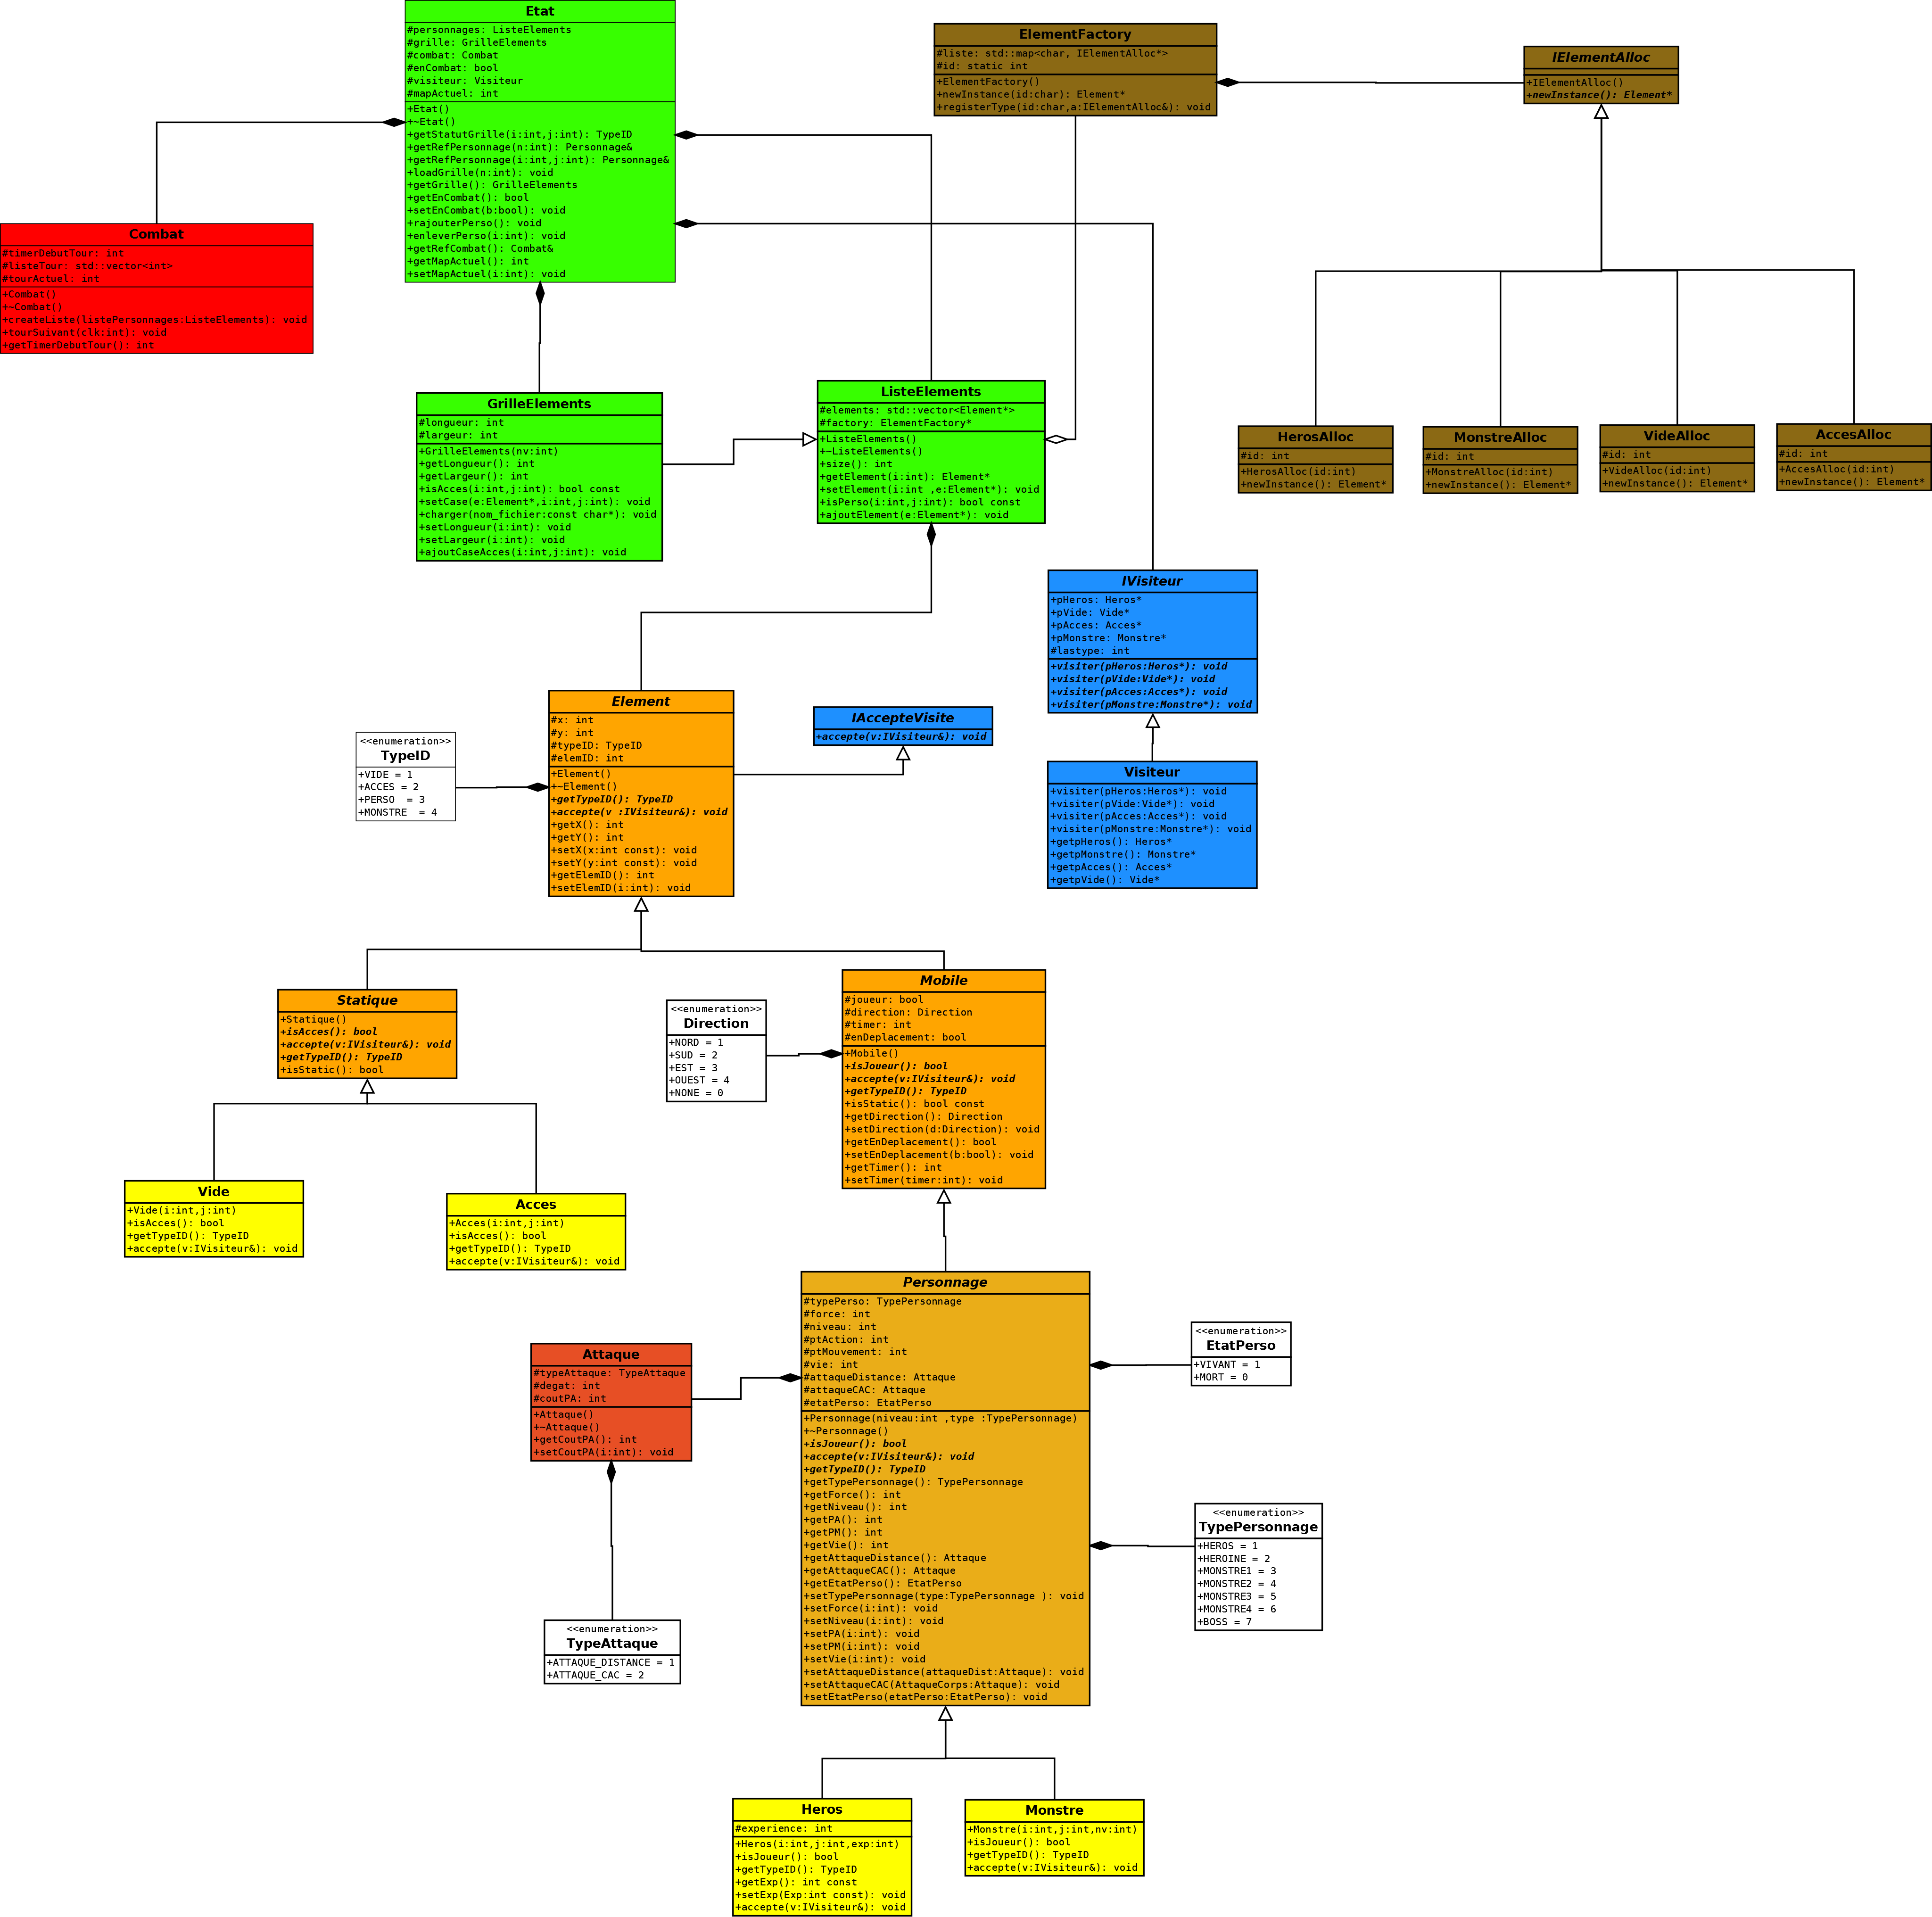
\includegraphics[scale=0.05]{img/state.png}
  \caption{\emph{Diagramme de classe du package etat du projet}}
\end{figure}


\end{document}